
\section{Kinetic Inductance Detectors}
\label{se:kids}


%\subsection{Presentation rapide des detecteurs}
%\subsection{Photometrie}
%\subsubsection{Rf}
%\subsubsection{Cf}
%
%\subsection{Non linearite par l'observation d'une source ponctuelle}

%%%%

\subsection{Description}

The theory of superconductivity described by \citep{PhysRev.108.1175} show that at low temperature, there is an attraction between electrons due to electron-phonon interactions that bind electrons together to form what we call Cooper pairs \citep{PhysRev.104.1189}. In superconductors this state is primarily responsible for superconductivity. When incident photons with sufficient energy are absorbed by the detector's superconducting film, they break Cooper pairs which increases the quasi-particles density and causes a change in the kinetic inductance $L_{K}$. The shift in the kinetic inductance $\delta L_{K}$ is proportional to the density of quasi-particles $\delta L_{K} \propto \delta n_{qp}$, which is directly proportional to the absorbed incident power : $\delta n_{qp} \propto \delta P_{opt}$.
Kinetic Inductance Detectors (KIDs) are RLC superconducting resonator introduced by \citep{2003Natur.425..817D} and that use this principle. Their resonant frequency is given by : 

\begin{equation}
f_{0} = \frac{1}{2\pi \sqrt{(L_{k}+L_{G})C(\varepsilon)}}, 
\end{equation}
 
where $L_{K}, L_{G}$ and $C$ are the resonator's kinetic inductance, geometric inductance and capacity. $\varepsilon$ is the material permittivity.
When a KID absorbs photons, its resonant frequency varies like :

\begin{equation}
\delta f_{0} = -\frac{1}{2}C(\varepsilon)f_{0}^{3} \delta L_{K}.
\end{equation}

A small change in the kinetic inductance results in a proportional shift of the resonant frequency. As a result, there is a linear relation between the absorbed optical power by the detector and the shift of the resonant frequency :

\begin{equation}
\delta f_{0} \propto -\delta P_{opt}.
\end{equation}

This is represented in Fig.~\ref{fig:resonance}. It si then possible to measure a flux variation on the sky by measuring the shift of resonant frequency of a detector. Two methods that are use to follow this shift are described further.

\begin{figure}
  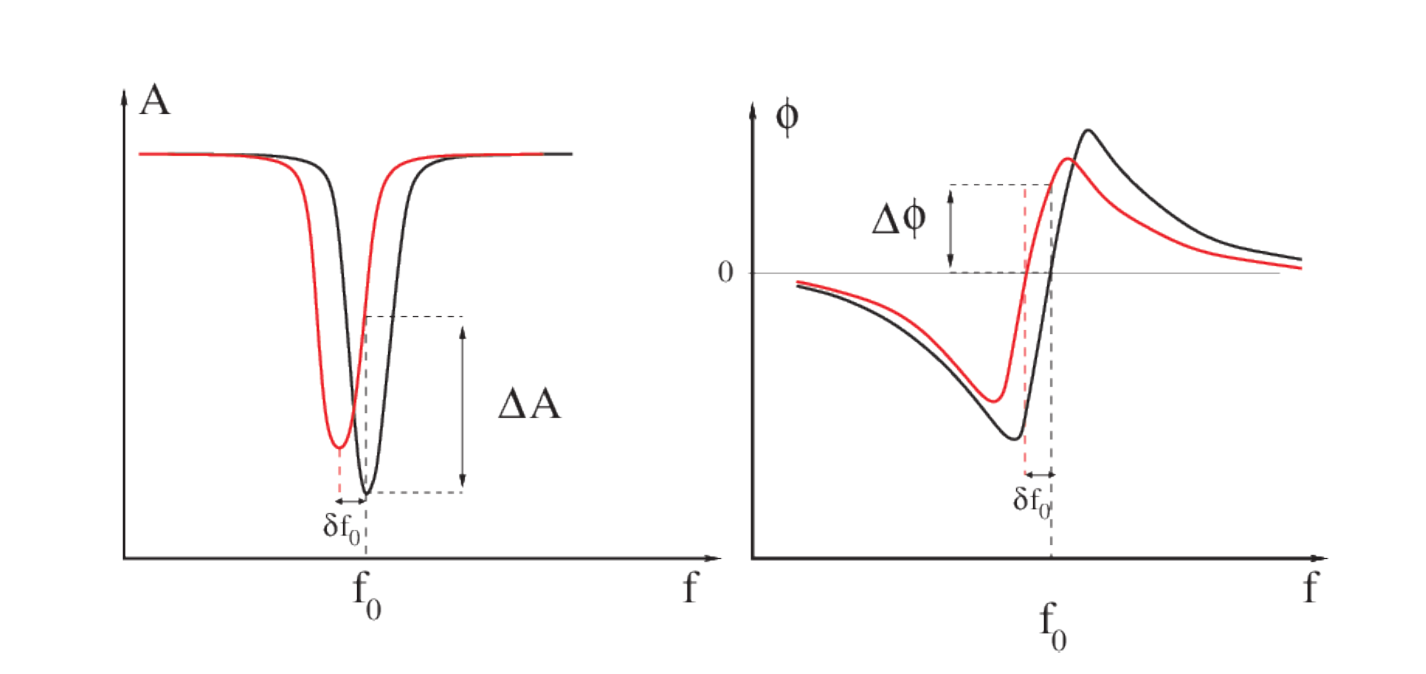
\includegraphics[clip, angle=0, width=\columnwidth]{Figures/resonance.png}
  %	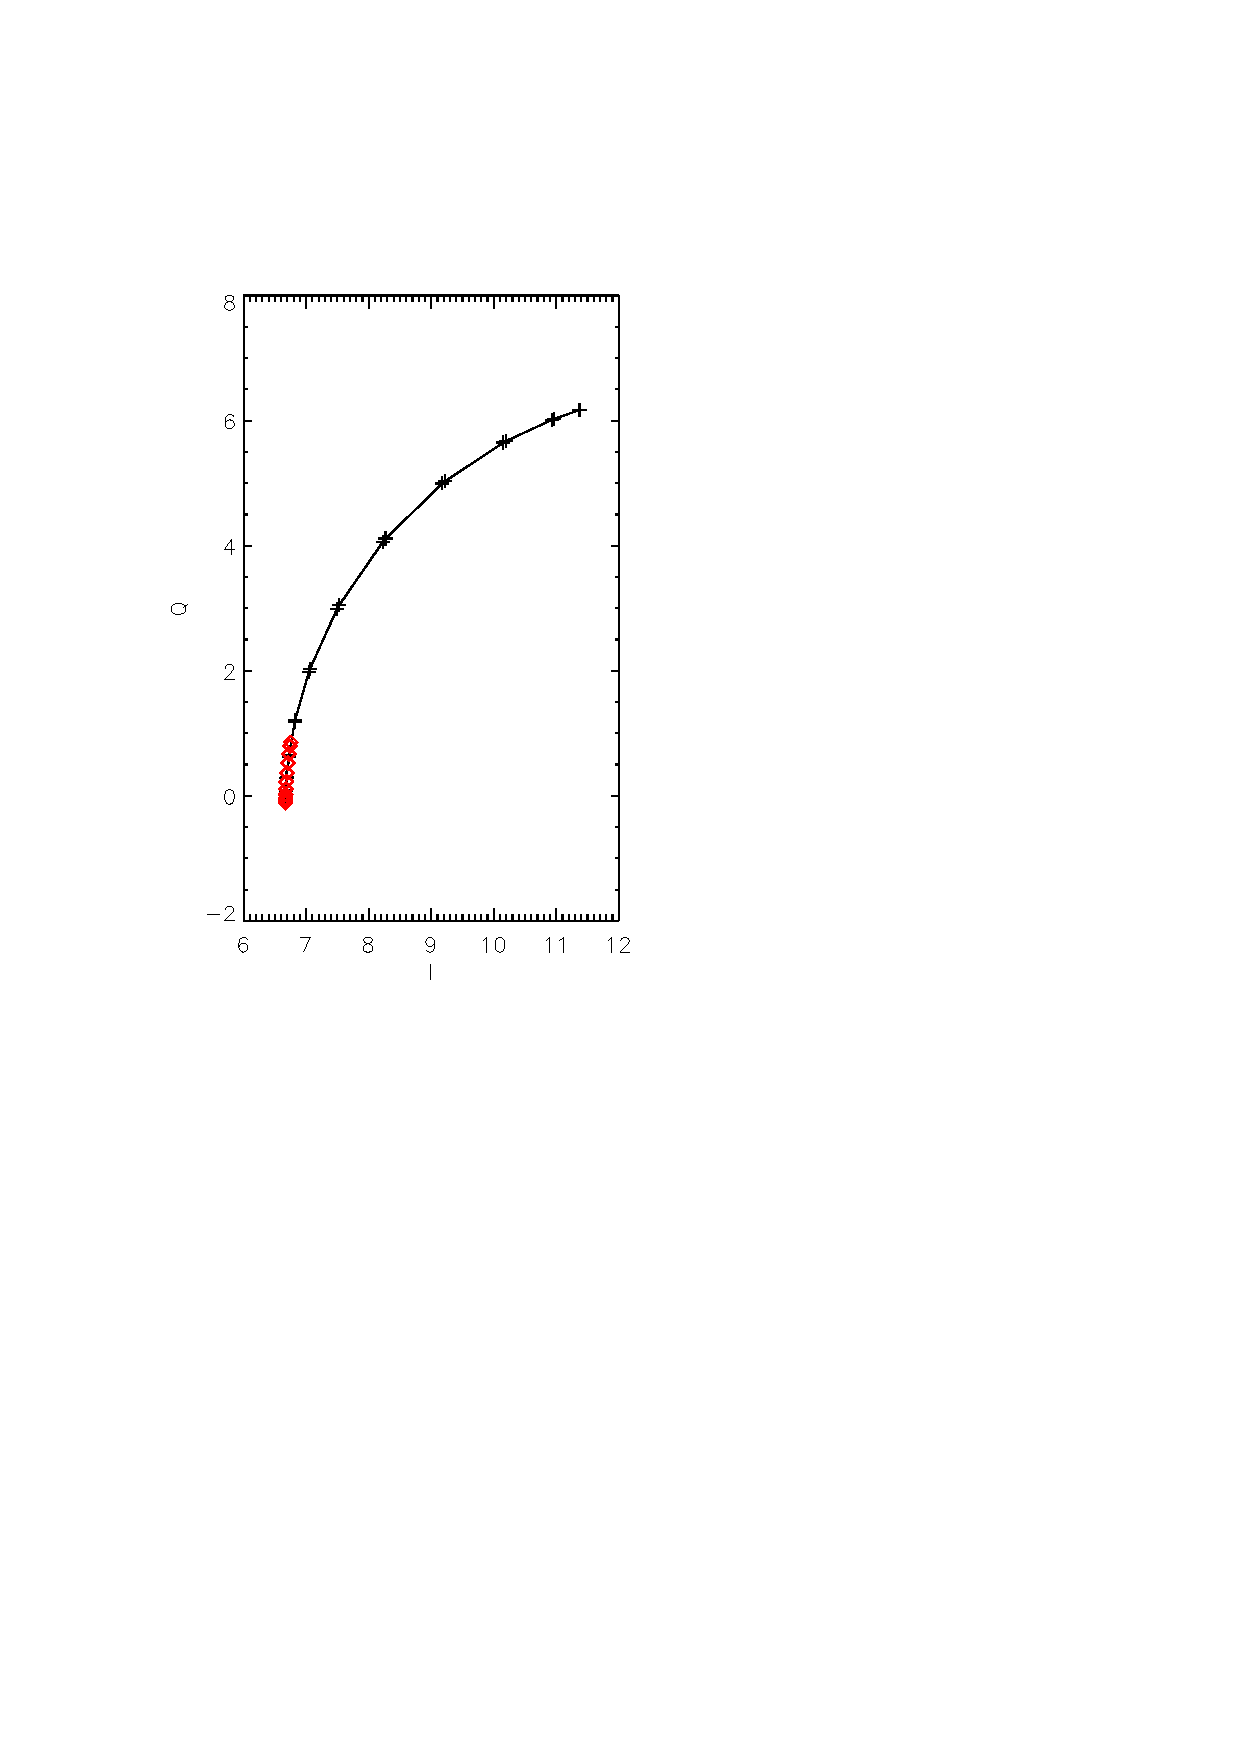
\includegraphics[clip, angle=0, width=\columnwidth]{Figures/resonance.pdf}
  \caption{Schematic representation of a KID resonance in amplitude (left) and phase (right), as a function of the excited tone injected in the feedline. The optical power absorbed by the detector is weak for black curves and increases for red curves. The absorption of a photon shifts the resonance frequency and this is directly proportional to the received power.}
  \label{fig:resonance}
\end{figure}


%Kinetic Inductance Detectors (KIDs) are RLC superconducting resonator, made from a thin metal film and introduced by \citep{2003Natur.425..817D}. They are based on a novel superconducting detector technology that provides high sensitivity and ease of multiplexing. 
%
%\citep{2016A&A...592A..26C} show that KID arrays behave appropriately in a space-like environment, they present short time constants making them less sensitive to cosmic rays compared to bolometers. This features make KIDs competitive with other technologies to be implemented in futur ground base or space CMB mission.
%In this section we give a brief summary of their main features and how photometry can be derived from their measurements, then we study the KID non-linearity, a systematic effect that must be taken into account in the design of futur experiments.
%
%This relation is linear for small variations in $P_{opt}$
%\citep{2010ApPhL..96z3511S}. 

\subsection{Transfer function}

A KID circuit is coupled to a transmission feedline that is expressed by the $S_{21}$ parameter. The KID transfer function reads : 

\begin{equation}
S_{21}(f) = \mathcal{I} +j\mathcal{Q} .
\end{equation}

\noindent where $\mathcal{I}$ and $\mathcal{Q}$ give respectively the real (in phase) and imaginary
(quadrature) of $S_{21}$. A model of a KID transfer function has been proposed
by \citet{2008ApPhL..93m4102G} :

\begin{equation}
S_{21} = \frac{2Z_{res}Z_{0}}{Z_{res}[2Z_{0} + j(X_{1}+X_{2})] + (Z_{0} +jX_{1})(Z_{0} +jX_{2})},
\end{equation}

with:

\begin{equation}
Z_{res} = \frac{Z_{0}Q_{e}}{2Q_{i}}[1 + 2jQ_{i}\frac{(f-f_{0})}{f_{0}}],
\end{equation}

\noindent where $X_{1}$, $X_{2}$, $Z_{0}$ are impedances, $Q_{i}$ is the
intrinsic quality factor of the resonator and $Q_{e}$ is the external quality
factor due to coupling with the measurement electronics. $f$ is the frequency of
excitation of the detector, and $f_{0}$ is the resonant frequency. Throughout
this paper, we shall assume typical values of KIDs $X_{1} = X_{2} =
0.5\,\Omega$, $Z_{0} = 50\,\Omega$, $Q_i=2\times 10^4$, $Q_e=10^4$ and $f_{0} =
1.8\times 10^9$\,Hz as measured on \nika\ and \nikad. The following section
addresses how the resonance of a KID is monitored and related to the incident
optical power.

% \section{Methods of signal reconstruction}
\subsection{Photometry}
\label{sec:signal}

A dedicated KID readout system has been developed by \citet{2013A&A...551L..12C}
and successfully used for \nika\ and \nika2\ \citep{2010A&A...521A..29M,2016JLTP..184..816C}. We here summarize its main charcteristics and the observables
that are relevant for our simulation work. We then present two ways to use them
to derive the photometry.

%% To convert the $\I(t)$ and $\Q(t)$ that
%% describe the resonance frequency shift $\delta f_0$ to the absorbed optical
%% power $\delta P_{opt}$. We have devised two ways to relate these
%% quantities. Both rely on a specific electronic modulation readout devised by
%% \citet{2013A&A...551L..12C} that we summarize first.

\subsubsection{Modulated readout technique}

\begin{figure}
  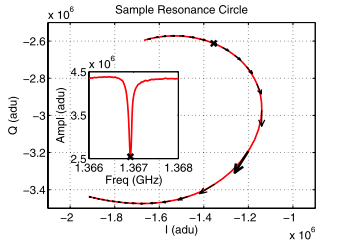
\includegraphics[clip,angle=0,width=\columnwidth]{Figures/resonance-circle.png}
  \caption{Trajectory of $\I$ and $\Q$ during a frequency sweep around the
    resonance of a KID. The arrows represent $(\di,
    \dq)$. \citep{2013A&A...551L..12C}}
  \label{circle-iq}
\end{figure}

The excitation tone frequency of a KID is modulated by a local oscillator with a
known frequency shift. This provides two values $f_{\pm} = f_0 \pm \delta
  f_{LO}/2$ with $\delta f_{LO} \simeq 1$\,kHz. Time ordered data values $(\mathcal{I}(t),\mathcal{Q}(t))$ are given by :

\begin{equation}
(\mathcal{I}(t), \mathcal{Q}(t)) = (\frac{\mathcal{I}(f_{+}) +
    \mathcal{I}(f_{-})}{2},
\frac{\mathcal{Q}(f_{+}) + \mathcal{Q}(f_{-})}{2}),
\end{equation}

and the differential values are :

\begin{equation}
\label{gradient}
(\frac{\di}{df}(t), \frac{\dq}{df}(t)) =
\left(\frac{\I(f_{+}) - \I(f_{-})}{\delta f_{LO}},
\frac{\Q(f_{+}) - \Q(f_{-})}{\delta f_{LO}}\right).
\end{equation}

These quantities are represented on Fig. \ref{circle-iq}. In this paper, we take
typical laboratory values and assume that $i$ and $q$ are sampled at
880\,Hz. This high acquisition rate is allowed by the sub-millisecond time
constant of the KIDs. For most experiments, such a high sampling rate is not
required and we average these measures over 40~samples to produce
four secondary quantities at 22\,Hz:

\begin{eqnarray}
\I  &=& \sum^{N_{m}=40}_{p=1} i_{p},\\
\Q  &=& \sum^{N_{m}=40}_{p=1} q_{p},\\
d\I &=& \sum^{N_{m}/2=20}_{p=1} i_{2p} - i_{2p-1},\\
d\Q &=& \sum^{N_{m}/2=20}_{p=1} q_{2p} - q_{2p-1}.
\end{eqnarray}

With these quantities in hand we have two methods to derive the transmitted
signal. They are presented in the following paragraphs.

\subsubsection{Method 1}
If a variation $\Delta\I(t)$, $\Delta\Q(t)$ is observed between successive ($\I$,
$\Q$) points, it is possible to estimate the shift of the resonant frequency
$\Delta f_{0}$ between these two samples by comparing ($\Delta \I$, $\Delta \Q$)
with the gradient $(\di,\dq)$ induced by the known and small $\delta
f_{0}$ of the local oscillator. This is done by a scalar projection of ($\Delta\I$,
$\Delta\Q$) on $(\di,\dq)$ that is tangent to the resonance circle. To have a
cleaner estimation of the latter, we take its running average over 50
points that we write $\langle . \rangle_{50}$ \citep{2014A&A...569A...9C}:

\begin{equation}
\label{eq:Rf}
\Delta f_{0} = \delta f_{LO} \frac{\Delta \I\, \langle \di
  \rangle_{50}
+ \Delta \Q\, \langle \dq \rangle_{50}}{\langle \di
  \rangle_{50}^{2}
 + \langle \dq \rangle_{50}^{2}},
\end{equation}

Note that this average is performed only on the tangent vector $(\di,\dq)$ so
that $\Delta f_0$ is sampled like $\I$ and $\Q$ at 22\,Hz. This method has been
successfully used in \nika\ and \nika2. Under large incoming power, the resonances can be shifted far from their excitation frequency. The $(\I, \Q)$ circle is then distorted and the tangent approximation of $(\di, \dq)$ no longer holds which can be the source of non-linearity. In the next paragraph we present an improved method to follow the shift of the resonant frequency.

\subsubsection{Method 2}

\begin{figure}
\includegraphics[clip, angle=0, width=\columnwidth]{Figures/circle_zres.eps}
\caption{Bottom: location of $\I$ and $\Q$ when a KID observes a point source of
  various fluxes. Top: ratio of the distance between $(\I,\Q)$ and the center of
  the fitted circle over the radius of this circle. All the points on the pure
  imaginary line at $\I=1$ are the result of the transformation of the circle
  into $Z_{res}$ according to eqs.~(\ref{eq:z_res}) and
  (\ref{eq:scale_rotate}).}
\label{fig:circle_zres}
\end{figure}

\todo{ref to the circular nature of (I,Q): \cite{2011ApJS..194...24M}}.\\

To improve method 1, we developed a new technique that fully exploits the circular
nature of the $(\I,\Q)$ trajectory, hereafter called \cf. It is
  based on the transformation property of a circle in the complex plane into a
  straight line. Indeed, let us consider a circle centered on $(0,1/2)$ with a
  radius of $1/2$ and compute its inverse:

\begin{eqnarray}
Z_{ref} &\equiv&\frac{1}{2} + \frac{1}{2}e^{i\phi}\,, \\
&=&\cos\frac{\phi}{2}e^{i\phi/2}\,,\\
Z_{res} &\equiv& 1/Z_{ref}\,, \label{eq:z_res} \\
&=&1-i\tan\frac{\phi}{2}\,.
\label{eq:z_res}
\end{eqnarray}

$Z_{res}$ is a straight line and along this line $Z$ varies linearly with
$\phi$ for small values of $\phi$. Experimentally, we are in this regime
when the signal is weak and when $\phi$ is defined w.r.t.~ the $(O,C)$ axis
as defined on Fig.~\ref{fig:circle_zres}. We thus fit the radius $r$ and the
center $(\I_c,\Q_c)$ of our measurement circle $Z=\I+j\Q$. Defining
$\alpha=\arctan\Q_c/\I_c$, we scale, rotate and translate this
circle to the $Z_{res}$ circle according to

\begin{equation}
Z_{ref} = \left(\begin{array}{c}
\I_{ref}\\
\Q_{ref}\end{array}\right) = 
\frac{-1}{2r}\left(\begin{array}{rr}
\cos\alpha & \sin\alpha\\
-\sin\alpha & \cos\alpha\end{array}\right)
\left(\begin{array}{c}
\I-\I_c\\
\Q-\Q_c\end{array}\right) +
\left(\begin{array}{c}
1/2\\
0\end{array}\right)
\label{eq:scale_rotate}
\end{equation}

The result of this transformation is shown on Fig.~\ref{fig:circle_zres}. A
variation of the signal $(\Delta\I,\Delta\Q)$ leads to a variation
$\Delta\phi$ along $Z$ that is proportional to the frequency shift $\Delta f$
that we are after to determine photometry. To derive the calibration between
these two quantities, we once again rely on the $(\di,\dq)$ that is induced by
the known $\delta f_{LO}$. Applying transformation (\ref{eq:scale_rotate}) to
$(\di,\dq)$, we obtain the corresponding variation $dy = Im(dZ_{res})$. The
final derivation of $\Delta f$ corresponding to $(\Delta\I,\Delta\Q)$ requires
the integration of $dy/\delta f_{LO}$. For the sake of simplicity, we fit
$Im(dZ_{res})$ as a polynomial of $dy/\delta f_{LO}$ that is therefore trivial
to integrate.

%% \begin{equation}
%% \tan\frac{\delta\phi}{2} \simeq \frac{\delta\phi}{2} +
%% \frac{(\delta\phi)^3}{15}
%% \end{equation}

\subsection{Non linearity characterization with simulations of observations of a point source}

\begin{figure}
\center
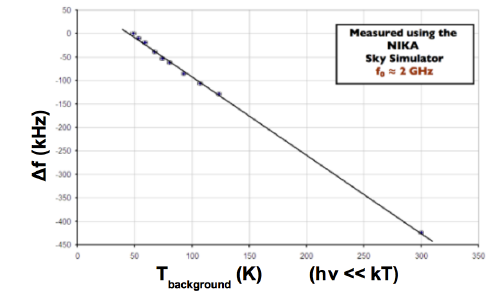
\includegraphics[clip, angle=0, width=\columnwidth]{Figures/KID-linearity-Monfardini2014.png}
\caption{KID linearity demonstrated in laboratory under realistic
  conditions. The plot shows the frequency shift of the resonance as a function
  of the optical background temperature (K). Solid line : linear fit of the
  experimental points. Credits : \citet{2014JLTP..176..787M}.}
\label{fig:KID-lin}
\end{figure}

Laboratory measurements with \todo{XXXX describe set up XXX} have shown that
KIDs are linear over a wide range of backgrounds (Fig.~\ref{fig:KID-lin}). However, for these measurements, $\Delta f$ was not reconstructed as described in the previous section, and we want to characterize our formalism up to $\epsilon$ of the order of $10^{-5}-10^{-6} $ TBC.

Non-linearity could appear as a consequence of too strong currents inside the resonator or to too strong induced magnetic fields leading to a loss of superconductivity \citep{Calvo2008} \todo{(articles Pippard, Parmenter ?)}. It can also arise when the source is very bright (such as planets of several tens of Jy) and the density of charge carriers is altered. This leads to $(\I,\Q)$ measures that leave the resonance circle, hence invalidating the approximations made in the photometric equations of the previous section. 
Another possible source of non linearity is the instrument scanning speed. Indeed, even if the source is moderately bright, if it is scanned too fast, $(\Delta\I,\Delta\Q)$ could be far from the tangent vector $(\di,\dq)$ which would alter their linear relation. Induced non-linearities in the two last cases result in a poor reconstruction of the shift of the resonant frequency. In principle this problem should be improved with the \cf\ method. In this paragraph, we explore the two last cases.\\

We simulate the measure of point source by a KID and show how linear this measure remains in various contexts. To characterize KIDs non linearity, we write the non linear detector response as :

\begin{equation}
m^{Rf,Cf} = m + \varepsilon m^2 +c_{0}.
\label{eq:model_kid_nl}
\end{equation}

$\varepsilon$ represents the non linearity of the KID.

We simulate the observation of a point source with a flux
that we vary between \todo{1 and 2000\,Jy TBC} (fluxes are unrealistically large on purpose for illustration). We assume that our instrument has
a 11\,arcsec FWHM Gaussian beam like the polarized 1\,mm channel of \nikad. We
also vary the scanning speed of our virtual instrument while keeping a minimum
of 3~samples per FWHM to respect the Nyquist criterion.
As shown in Fig.~\ref{fig:planet_profiles} and Fig.~\ref{fig:flux_out_vs_in}, non linearity appears with the distortion of the input gaussian profile in the case of method 1\ method whereas \cf\ remains linear on the same flux scale.

\begin{figure}
  \includegraphics[clip, angle=0, width=\columnwidth]{Figures/planet_profiles.eps}
  \caption{Comparison of an incoming flux that we vary between 1 and 2000 Jy TBC (in black), with flux reconstructed by method 1\ and \cf. Fluxes are unrealistically large on purpose for illustration. }
  \label{fig:planet_profiles}
\end{figure}


\begin{figure}
  \includegraphics[clip, angle=0, width=\columnwidth]{Figures/flux_out_vs_in.eps}
  \caption{Comparison of an incoming flux that we vary between 1 and 2000 Jy TBC (in black), with flux reconstructed by method 1\ and \cf. Fluxes are unrealistically large on purpose for illustration. }
  \label{fig:flux_out_vs_in}
\end{figure}

For all simulations we computed the non-linearity coefficient $\varepsilon$ from eq.~\ref{eq:model_kid_nl} by doing a fit of the input fluxes as a fonction of output fluxes. Results are shown in Tab.~\ref{tab:eps}. As in the two figures the non-linearity coefficients show method 1\ method is less linear than \cf\ on the same flux scale.\\

\begin{table}
\center
\begin{tabular}{|c|c|c|}
	\hline
	    & $\frac{3pts}{beam}$ & $\frac{5pts}{beam}$ \\
	\hline
method 1\	&  $-4.58 \times 10^{-5}$ & $-2.33 \times 10^{-5}$ \\
	\hline
\cf\ & $1.09 \times 10^{-7}$   & $8.90 \times 10^{-8}$ \\
	\hline
\end{tabular}
\caption{Non-linearity coefficients $\varepsilon$ from an incoming flux that we vary between 1 and 500 Jy.}
\label{tab:eps}
\end{table}


KIDs are a novel technology successfully used in \nikad . Because of their multiplexing capability and their short time constant, they are one of the best candidates to be implemented on experiments that need larger arrays. In this section we studied KIDs non-linearity and its impact on CMB B mode measures, considering the brightness of a source, the scanning speed of the instrument and the method that we use to follow the shift of the resonant frequency and retrieve the absorbed power.
Simulations of a KID exposed to a point source with a large variation of fluxes have shown that as expected, the brighter is the source, the more non-linearities appear due to a poor reconstruction of the resonant frequency. Although both reconstruction methods give good results, \cf\ remains more linear at high fluxes than method 1 . Plus, KID non-linearity should not impact measures of CMB B modes, in fact the non-linearity coefficients that we found are in the range of $[10^{-5} - 10^{-8}]$, so it meets the requirement addressed in Sec.\ref{sec:cmb}.
In futur CMB polarization experiments, the use of a half wave plate more and more common. It presents a lot of advantages, but can also be source of various systematic effects. In the next section we will address the non-linearity that can arise from rotating a half wave plate in an instrument.
